\section{Code Validation}
A set of simulations was performed to ensure the accuracy and reliability of omnisoot for prediction of soot formation. Aerosol dynamics is validated by comparing the results of population balance models implemented in omnisoot with those of DEM simulations from literature. Carbon and hydrogen mass and energy balance is also rigorously evaluated to ensure that residuals fall within the bounds of acceptable numerical error.





\subsection{Coagulation}
A test case was designed and conducted to validate the coagulation sub model of both particle dynamics models, MPBM and SPBM, by comparing the results of omnisoot with those of DEM~\citep{kholghy2021surface}. The constant volume reactor was used for this test case, but it will be applicable to other reactors and flame models as long as the particle residence time matches with the values obtained by DEM. An adiabatic reactor with the volume of 1 $\mathrm{m^3}$ is initialized with $2.6261\times10^{18}$ spherical particles 2 nm in diameter. The initial conditions are indicated in Table~\ref{tab:simcond_coagtest}. The particles are allowed to coagulate in the free molecular regime and grow in size while no inception, PAH adsorption and surface growth occur. Figure~\ref{fig:coagvalid_Nd} demonstrates ${N_{agg}}$, ${N_{pri}}$, ${d_m}$, ${d_g}$ of particles obtained by omnisoot that are in good agreement with DEM results~\citep{kholghy2021surface}. ${N_{pri}}$ is conserved during coagulation resulting in identical flat lines for both particle dynamics models, but ${N_{agg}}$ declines over time with the higher decay rate for SPBM because it accounts for the polydispersity of agglomerates that results in larger collision frequency compared to MPBM. Therefore, mean mobility and gyration diameter  of SPBM (red lines in Figure~\ref{fig:coagvalid_Nd}b) are slightly larger than those of MPBM (blue line of the same figure).

\begin{figure}[H]
	\centering
	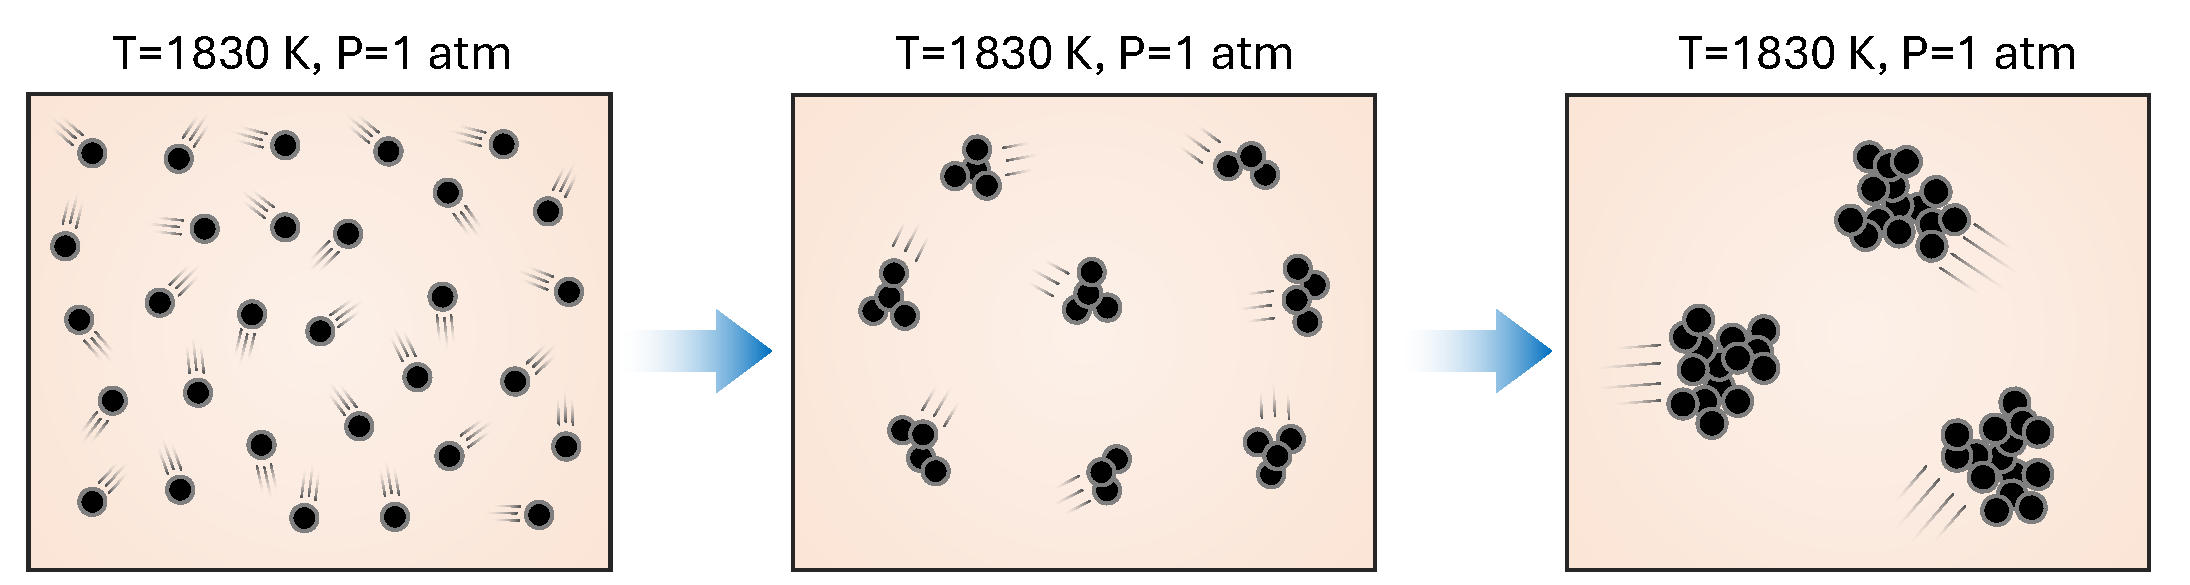
\includegraphics[width=0.9\textwidth]{Figures/Results/Validation/Coagulation/coagulation_scheme.pdf}
	\caption{The schematic of agglomeration process in the coagulation test cases where initially spherical particle collide and form agglomerate}
	\label{fig:coagscheme}
\end{figure}

MPBM model cannot resolve PSD because of the monodispersity assumption. In contrast, SPBM tracks the number concentration of particles in separate sections that can be used to construct evolving PSD and calculate mean properties and determine the spread of size distribution of particles during coagulation. Figure~\ref{fig:coagvalid_sigmapsd}a shows the standard deviation of mobility diameter, ${\sigma_g}$, predicted by SPBM in close agreement with DEM results. ${\sigma_g}$ starts from unity indicating a monodisperse population at the beginning of simulation, and it finally reaches 2.03 that is the signature standard deviation of the free molecular regime~\citep{vemury1995self}. Figure~\ref{fig:coagvalid_sigmapsd} demonstrates the evolution of non-dimensional PSD from $t=$1 ms to 677 ms. The PSD is plotted for the normalized concentration, ${\Psi= \bar{v}n_{agg}(v,t)/N_{agg,\infty}}$ and dimensionless volume, ${\eta= v/ \bar{v}}$, where ${n_{agg}(v,t)}$ is the size distribution function of agglomerate, ${v}$ particle volume, ${\bar{v}}$ mean particle volume, ${N_{agg,\infty}}$ total number concentration of agglomerates. For short residence times, $t\approx$4 ms, the PSD resembles a half bell curve because the majority of particles has sizes close to ${d_0=}$2 nm with the average volume close to the minimum volume, so the particles with ${\eta\approx1}$ has the largest concentration. As particles grow by coagulation, the PSD rapidly transitions to a full bell-curve ($\mathrm{t\ge}$22 ms) and does not change for longer residence times, $\mathrm{t\ge}$447 ms marking the attainment of SPSD in a good agreement with DEM results. This confirms the capability of SPBM implemented in omnisoot to capture SPSD for soot agglomerates as a signature of Brownian-driven particle coagulation.  

\begin{table}
	\caption{The simulations conditions of the coagulation test case~\citep{kholghy2021surface}}
	\label{tab:simcond_coagtest}
	\centering
	\begin{tabular}{l l}
		\hline
		\textbf{Property} & \textbf{Value} \\
		\hline
		Composition & $\mathrm{CH_4}$:0.425, $\mathrm{O_2}$:0.435, $\mathrm{N_2}$:0.14\\
		T & 1830 K\\
		P & 1 atm \\
		${N^1_{agg}}$ & $3.514\times10^{-5} \mathrm{mol/kg}$ \\ 
		${N^1_{pri}}$ & $3.514\times10^{-5} \mathrm{mol/kg}$\\
		${d^1_{p}}$ & 2 nm \\
		\hline
	\end{tabular}
\end{table}


\begin{figure}[H]
	\centering
	\begin{subfigure}[t]{0.4\textwidth}
		\begin{tikzpicture}
			\draw (0, 0) node[inner sep=0] 	{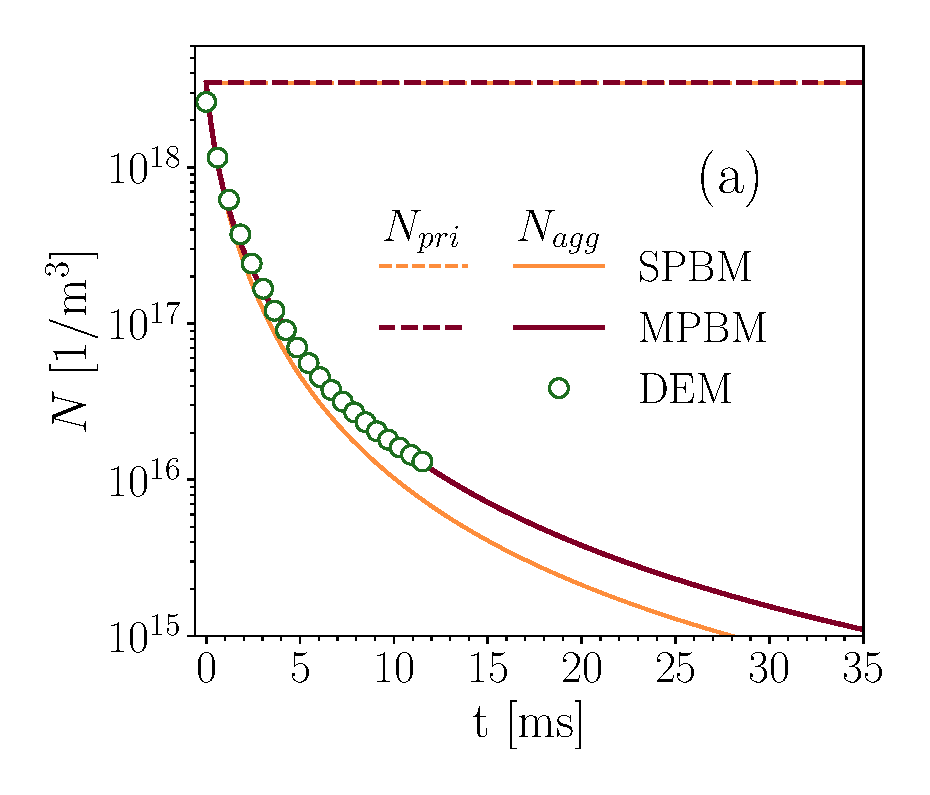
\includegraphics[width=1\textwidth]{Figures/Results/Validation/Coagulation/N_agg_pri.pdf}};
			\draw (2.1, 0.03) node {\scriptsize{\cite{kholghy2021surface}}};
		\end{tikzpicture}
	\end{subfigure}
	\begin{subfigure}[t]{0.4\textwidth}
		\begin{tikzpicture}
			\draw (0, 0) node[inner sep=0] 	{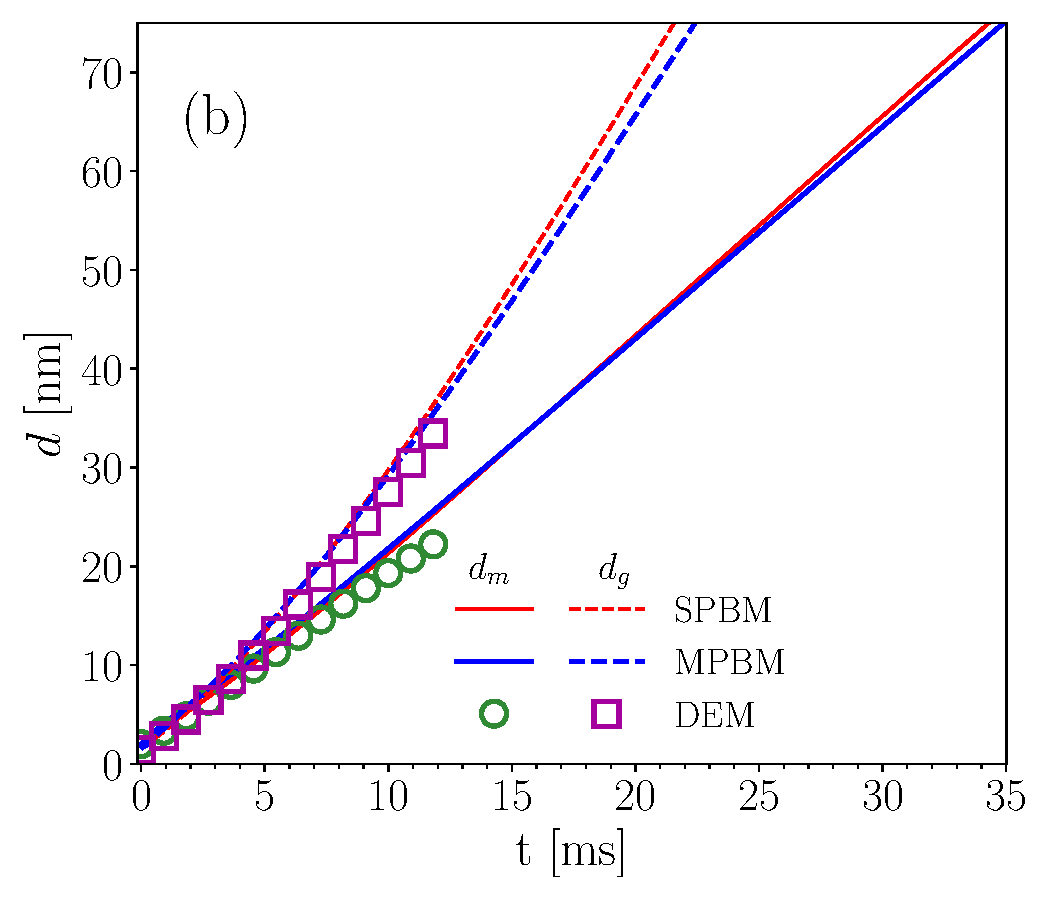
\includegraphics[width=1\textwidth]{Figures/Results/Validation/Coagulation/d_mg.pdf}};
			\draw (2.2, -1.22) node {\scriptsize{\cite{kholghy2021surface}}};
		\end{tikzpicture}
	\end{subfigure}
	\caption{The total number concentration of agglomerates and primary particles (a), and mobility and gyration diameter (b) obtained with omnisoot using MPBM and SPBM that are in close agreement with the DEM results~\citep{kholghy2021surface} indicating the validation of coagulation sub-model}
	\label{fig:coagvalid_Nd} 
\end{figure}


%\begin{figure}[H]
%	\centering
%	\begin{subfigure}[t]{0.4\textwidth}
%		\centering
%		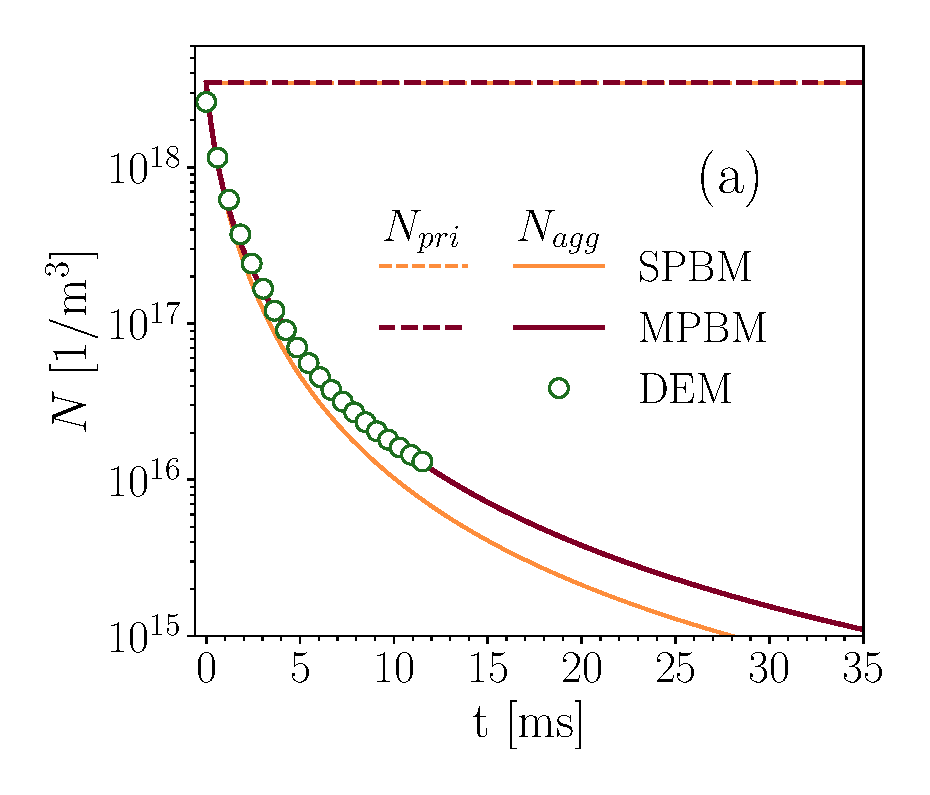
\includegraphics[width=1\textwidth]{Figures/Results/Validation/Coagulation/N_agg_pri.pdf}
%	\end{subfigure}
%	\begin{subfigure}[t]{0.4\textwidth}
%		\centering
%		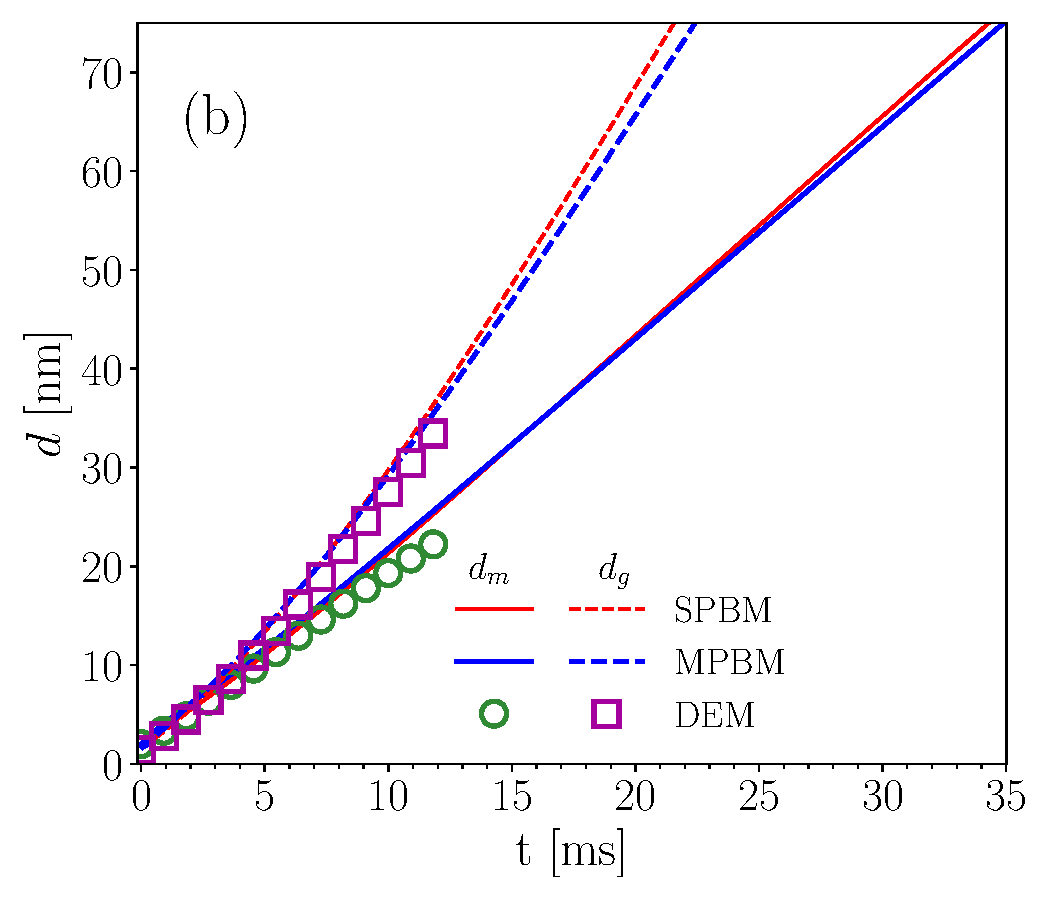
\includegraphics[width=1\textwidth]{Figures/Results/Validation/Coagulation/d_mg.pdf}
%	\end{subfigure}
%	\caption{The total number concentration of agglomerates and primary particles (a), and mobility and gyration diameter (b) obtained with omnisoot using MPBM and SPBM that are in close agreement with the DEM results~\citep{kholghy2021surface} indicating the validation of coagulation sub-model}
%	\label{fig:coagvalid_Nd}
%\end{figure}


%\begin{figure}[H]
%	\centering
%	\begin{subfigure}[t]{0.4\textwidth}
%		\centering
%		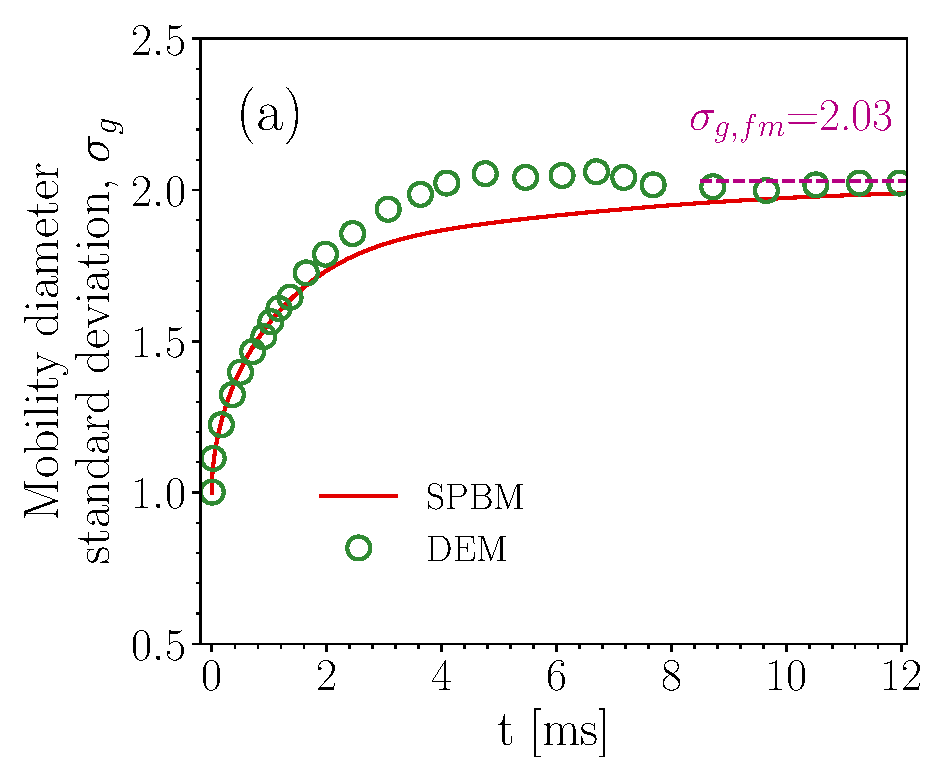
\includegraphics[width=1\textwidth]{Figures/Results/Validation/Coagulation/sigmag.pdf}
%	\end{subfigure}
%	\begin{subfigure}[t]{0.4\textwidth}
%		\centering
%		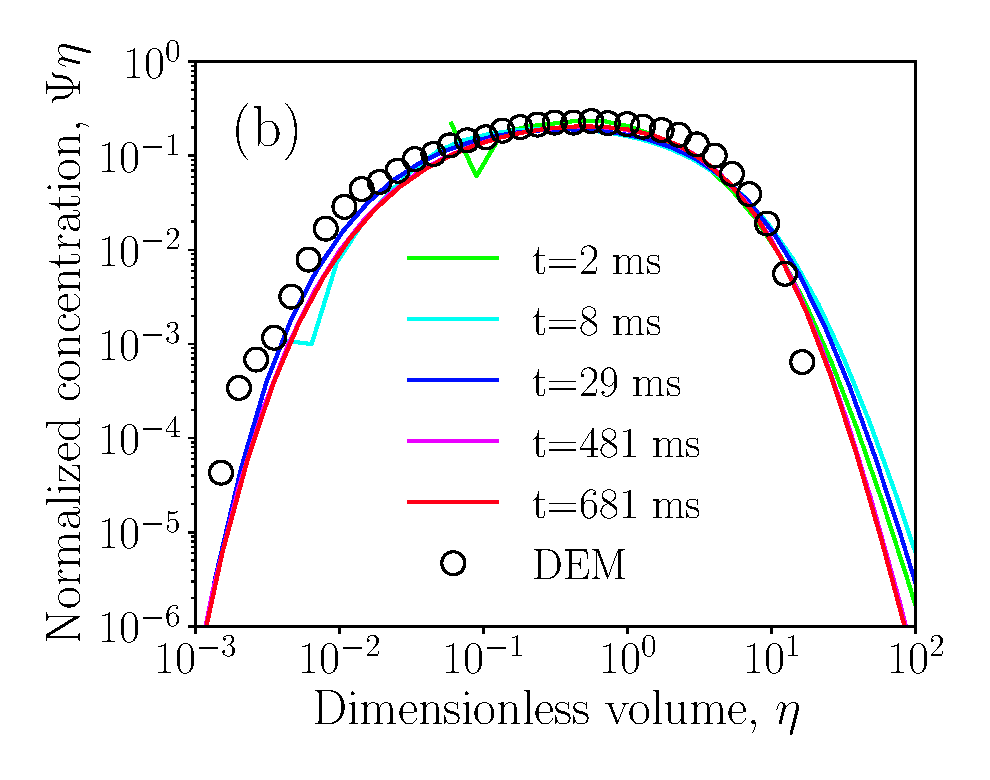
\includegraphics[width=1\textwidth]{Figures/Results/Validation/Coagulation/PSD.pdf}
%	\end{subfigure}
%	\caption{The standard deviation of mobility diameter, $\mathrm{\sigma_g}$ obtained with SPBM in close agreement with DEM results~\citep{kholghy2021surface} (left pane) that reaches $\mathrm{\sigma_{g,fm}=2.03}$ characteristic of the free molecular regime~\citep{vemury1995self}; the particle size distribution (normalized number concentration of agglomerates is plotted against non-dimensional volume in the right pane) at different residence times that overlaps after initial transient phase marking the attainment of self-preserving size distribution}
%	\label{fig:coagvalid_sigmapsd}
%\end{figure}


\begin{figure}[H]
	\centering
	\begin{subfigure}[t]{0.4\textwidth}
		\begin{tikzpicture}
			\draw (0, 0) node[inner sep=0] 	{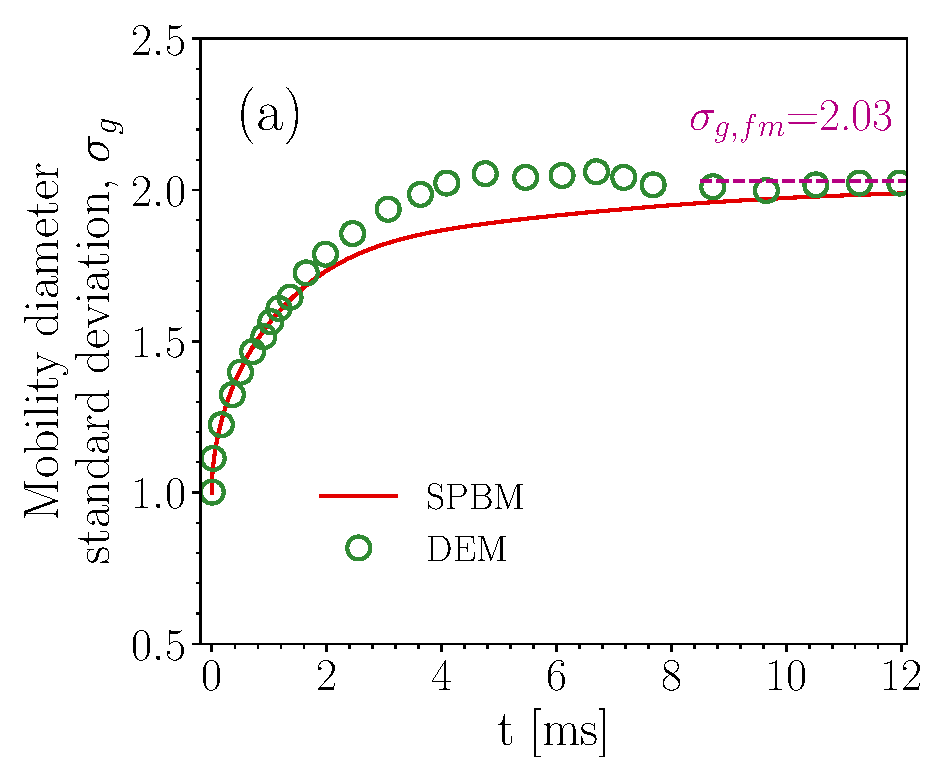
\includegraphics[width=1\textwidth]{Figures/Results/Validation/Coagulation/sigmag.pdf}};
			\draw (0.52, -0.86) node {\scriptsize{\cite{kholghy2021surface}}};
		\end{tikzpicture}
	\end{subfigure}
	\begin{subfigure}[t]{0.4\textwidth}
		\begin{tikzpicture}
			\draw (0, 0) node[inner sep=0] 	{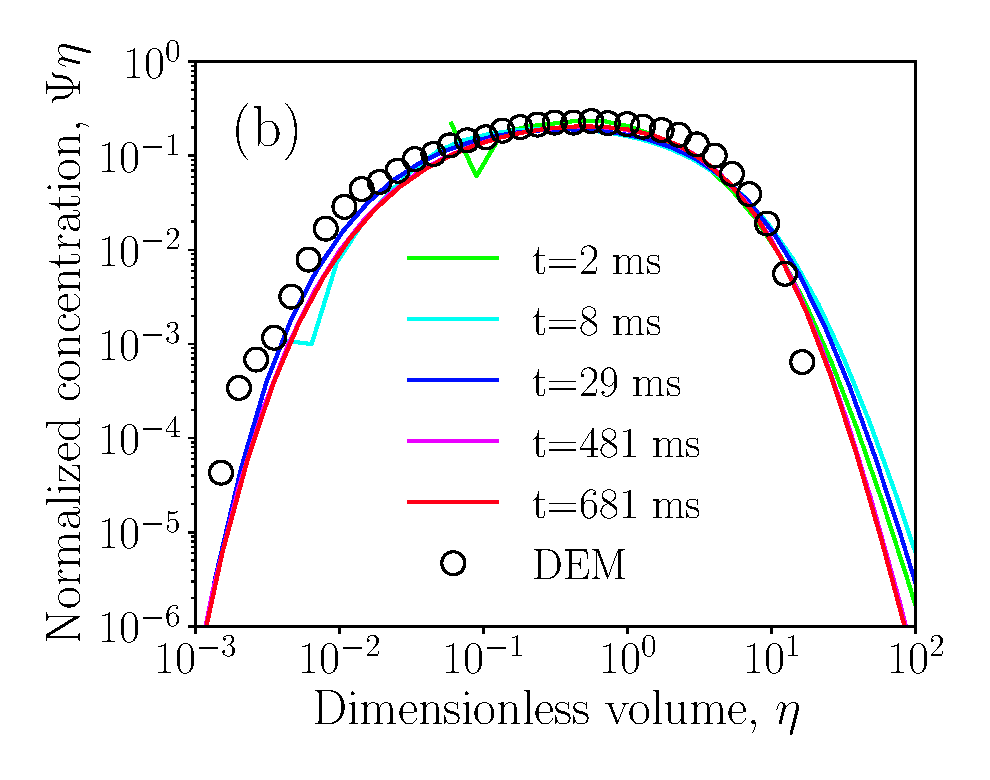
\includegraphics[width=1\textwidth]{Figures/Results/Validation/Coagulation/PSD.pdf}};
			\draw (1.12, -1.12) node {\scriptsize{\cite{goudeli2015coagulation}}};
		\end{tikzpicture}
	\end{subfigure}
	\caption{The standard deviation of mobility diameter, $\mathrm{\sigma_g}$, obtained with SPBM in close agreement with DEM results~\citep{kholghy2021surface} (shown in the left pane) that reaches $\mathrm{\sigma_{g,fm}=2.03}$ characteristic of the free molecular regime~\citep{vemury1995self}; the particle size distribution normalized number concentration of agglomerates is plotted against non-dimensional volume (shown in the right pane) at different residence times that overlaps after initial transient phase marking the attainment of self-preserving size distribution in good agreement with DEM results~\citep{goudeli2015coagulation}}
	\label{fig:coagvalid_sigmapsd} 
\end{figure}

\subsection{Elemental and Energy Balance Assessment}

\noindent To ensure the accuracy and reliability of the simulations, the conservation of elemental mass and energy was assessed across all reactor models implemented in {omnisoot}. Elemental balances of carbon and hydrogen, as well as the total energy (internal or enthalpy depending on the reactor type) of the gas-particle system, were evaluated during soot formation processes under various pyrolysis and combustion conditions.
Simulations were performed using different combinations of PAH growth and particle dynamics models, and the relative errors in elemental and energy balances were monitored over time or reactor length. The residuals for all reactor configurations remained within acceptable limits (typically below $10^{-10}$), confirming that {omnisoot} accurately preserves mass and energy during the coupled evolution of gas-phase and particulate species. Figure~\ref{fig:constuvvalid} demonstrates the relative error of total carbon, hydrogen and energy in a CVR simulation for the pyrolysis of 30\% $\mathrm{CH_4}$-$\mathrm{N_2}$ with the initial temperature and pressure of 2455 K and 3.47 atm. The relative errors are less than $10^{-11}$ for different combinations of PAH growth and particle dynamics models. The same evaluation was performed for CPR, PSR and PFR reactor and the corresponding residuals are shown in Figures~\ref{fig:cprvalid}-\ref{fig:pfrvalid}.

%\subsubsection{Constant Volume Reactor}
%The pyrolysis of 30\% $\mathrm{CH_4}$ diluted in $\mathrm{N_2}$ with the initial temperature and pressure of 2455 K and 3.47 atm, respectively, was simulated using CVR model for the residence time of 40 ms. The combination of available PAH growth and particle dynamics models leads to eight different cases that were simulated to ensure the conservation of mass and energy. Here, we focus on the total elemental balance of carbon and hydrogen because they are involved in soot processes. %The validity of models are evaluated based on relative error based on the initial mass and energy of gas. 
%Figure~\ref{fig:constuvvalid} demonstrates the relative error of total carbon, hydrogen and energy of system for different PAH growth and particle dynamics models in the constant pressure reactor that is less than $\mathrm{10^{-10}}$ for all parameters confirming the validity of model in satisfying the mass and energy balance.

\begin{figure}[H]
	\centering
	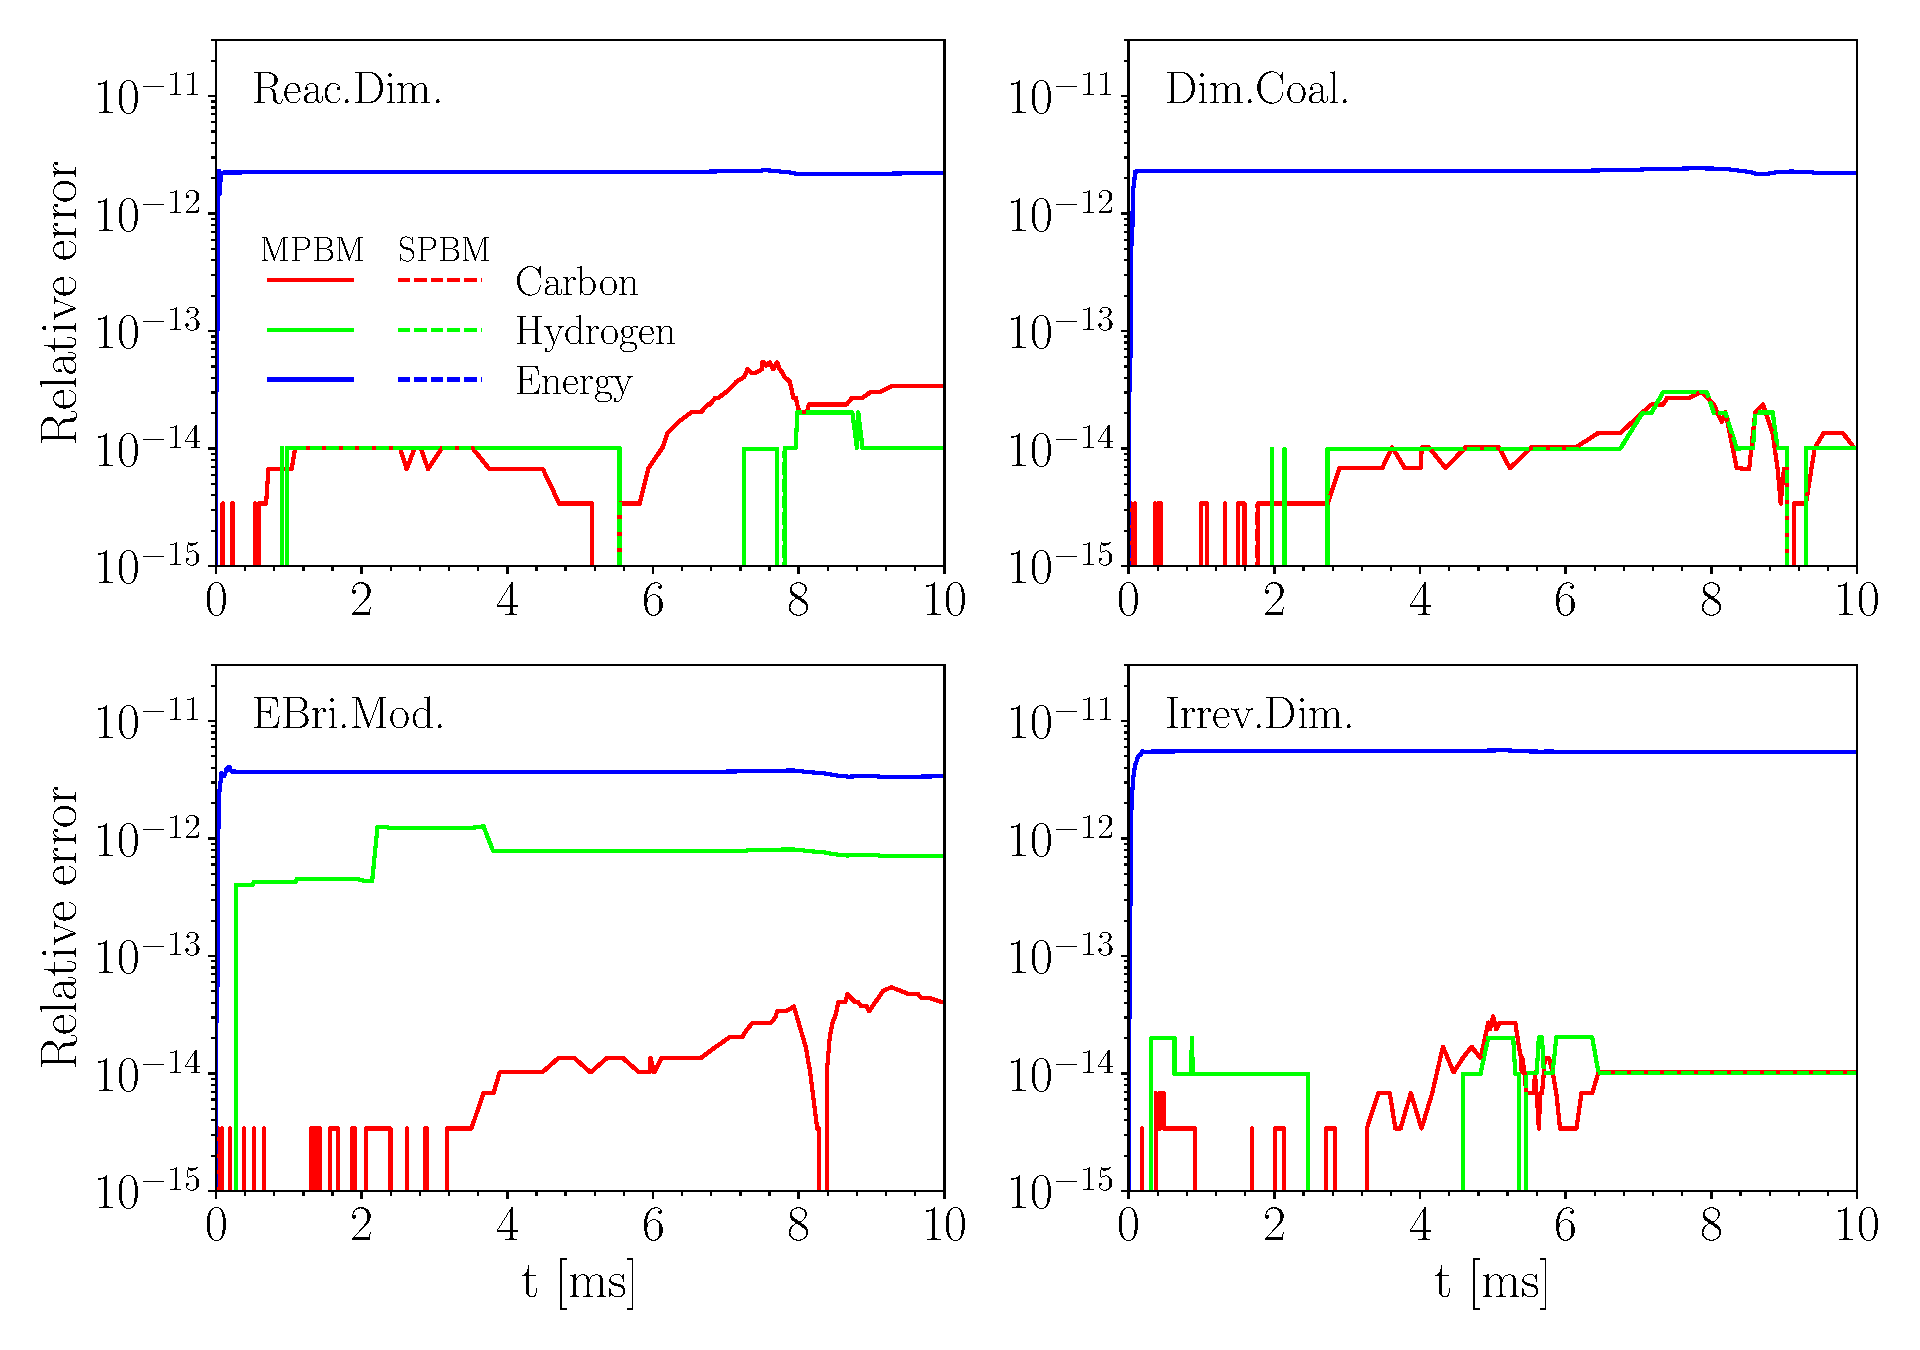
\includegraphics[width=0.8\textwidth]{Figures/Results/Validation/ConstUV/relerr_constuv.pdf}
	\caption{The relative error (residual) of total carbon (red line) and hydrogen (green line) mass, and total internal energy residual of gas and soot (blue line) plotted against residence time during pyrolysis of 30\% $\mathrm{CH_4}$-$\mathrm{N_2}$ at 2455 K and 3.47 atm in CVR simulated using different PAH growth models along with MPBM (solid line) and SPBM (dashed line).}
	\label{fig:constuvvalid}
\end{figure}



